\documentclass[aspectratio=169]{beamer}

%=======================
%       IMPORTS
%=======================

\usepackage{amsmath, amsthm, amssymb}   % Math symbols, environments etc.
\usepackage{mathtools}
\usepackage{fontspec}                   % For Unicode fonts
\usepackage{unicode-math}               % For Unicode math fonts
\usepackage{microtype}                  % Nicer interword spacing
\usepackage{polyglossia}                % Provides locale-specific formatting
\usepackage{csquotes}
\usepackage{svg}                        % For including SVG files
\usepackage{booktabs}                   % Nicer tables
\usepackage{tabularx}                   % Allows for linebreaks in tables

\usepackage[
    backend = biber
]{biblatex}

\addbibresource{quaternionen.bib}

% Set beamer theme
\usetheme{metropolis}
% \beamertemplatenavigationsymbolsempty
\metroset
{
    sectionpage = simple,
    subsectionpage = simple
}

\setbeamertemplate{caption}{\raggedright\insertcaption\par}

\usecolortheme{rose}

\setbeamercolor{quote}{fg=black!80!white, bg=blue!10!white}

\setmathfont{TeX Gyre Pagella Math}
\setmonofont[Scale=0.9]{Fira Mono}
\setmathfont[range=\setminus]{Asana Math}

\newfontfamily{\mathroman}{TeX Gyre Pagella}[Scale=MatchUppercase]

% Language Setup
\setdefaultlanguage[spelling=new, babelshorthands=true]{german}

% Set path for graphics
\graphicspath{{./graphics/}}

% hyperref setup
\hypersetup
{
    pdfencoding = auto      % For umlauts in PDF sections
}

%=======================
%    CUSTOM COMMANDS
%=======================
\newcommand{\Ham}{\ensuremath{\mathbb{H}}{ }}
\newcommand{\R}{\ensuremath{\mathbb{R}}{ }}
\newcommand{\diff}[2]{\ensuremath{\frac{\partial #1}{\partial #2}}}
\newcommand{\lap}[2]{\ensuremath{\frac{\partial^2 #1}{\partial #2^2}}}
\newcommand{\half}{\frac{1}{2}}

\DeclarePairedDelimiter\abs{\lvert}{\rvert}

\DeclareMathOperator{\spur}{spur}
\DeclareMathOperator{\kernel}{kern}
\DeclareMathOperator{\Mat}{Mat}
\DeclareMathOperator{\End}{End}
\DeclareMathOperator{\grad}{grad}
\DeclareMathOperator{\newdiv}{div}
\DeclareMathOperator{\rot}{rot}

\newtheorem{cor}{Korollar}

%=======================
%  DOCUMENT INFORMATION
%=======================

\title{\textsc{Hamilton}sche Quaternionen}
\subtitle{Proseminar Mathematik}
\author[L.~Richardt]{Leon Richardt}
\date[2020-07-07]{7. Juli 2020}
\institute{Universität Osnabrück}

\begin{document}

    \nocite{ebbinghaus_zahlen_1992}

    \begin{frame}
        \titlepage
    \end{frame}

    \begin{frame}{Überblick}
        \tableofcontents
    \end{frame}

    \section{Reelle Algebren}
    \begin{frame}
        \begin{block}{Anmerkung}
            In dieser Präsentation stehen kleine griechische Buchstaben stets für reelle Zahlen; lateinische Buchstaben stehen für Elemente der momentan betrachteten Algebra.
        \end{block}
    \end{frame}

    \begin{frame}
        \begin{definition}
            Ein Vektorraum \(V\) über \R mit einer Produktabbildung
            \[
                V \times V \to V, (x, y) \mapsto xy
            \]
            heißt \textbf{Algebra} über \R (oder reelle Algebra), wenn die beiden Distributivgesetze
            \begin{gather*}
                (\alpha x + \beta y) z = \alpha \cdot xz + \beta \cdot yz, \\
                x (\alpha y + \beta z) = \alpha \cdot xy + \beta \cdot xz
            \end{gather*}
            für alle \(\alpha, \beta \in \R\) und \(x, y, z \in V\) erfüllt sind.
        \end{definition}
    \end{frame}

    \begin{frame}
        \begin{definition}
            Ein Element \(x\) einer Algebra \(\mathcal{A}\) heißt \textit{Nullteiler}, falls es ein Element \(0 \neq y \in \mathcal{A}\) mit \(xy = 0\) oder \(yx = 0\) gibt.

            Konsequenterweise heißt eine Algebra \textit{nullteilerfrei}, falls sie keine Nullteiler \(\neq 0\) besitzt.
        \end{definition}
    \end{frame}

    \begin{frame}
        \begin{definition}
            Eine Algebra \(\mathcal{A} = (V, \cdot)\) heißt \dots
            \begin{itemize}
                \item
                    \dots{} \textit{assoziativ}, wenn \(x(yz) = (xy)z\) für alle \(x, y, z \in V\) gilt.
                \item
                    \dots{} \textit{kommutativ}, wenn \(xy = xy\) für alle \(x, y \in V\) gilt.
                \item
                    \dots{} \textit{mit Einselement}, wenn es ein Element \(e \in V\) mit \(ex = xe = x\) für alle \(x \in V\) gibt.

                \item
                    \dots{} \textit{Divisionsalgebra}, falls \(\mathcal{A} \neq 0\) und die Gleichungen
                    \[
                        ax = b \text{ und } ya = b
                    \]
                    für alle \(a, b \in V, \, a \neq 0,\) eindeutig lösbar sind.
            \end{itemize}
        \end{definition}
    \end{frame}

    \begin{frame}
        \begin{lemma}
            Folgende Aussagen über eine endlichdimensionale Algebra \(\mathcal{A}\) sind äquivalent:
            \begin{itemize}
                \item[i)]
                    \(\mathcal{A}\) ist Divisionsalgebra.

                \item[ii)]
                    \(\mathcal{A}\) ist nullteilerfrei.
            \end{itemize}
        \end{lemma}
    \end{frame}

    \begin{frame}
        \begin{proof}
            i) \(\implies\) ii) ist klar.

            ii) \(\implies\) i): \\
            Sei \(a \in \mathcal{A} \setminus \{0\}\).
            Die Abbildung \(\varphi \colon \mathcal{A} \to \mathcal{A},\, x \mapsto ax\) ist ein VR-Endomorphismus.
            Wegen der Nullteilerfreiheit ist \(\kernel(\varphi) = \left\{ 0 \right\}\), was aufgrund des Kernkriteriums die Injektivität bedeutet.
            Da weiterhin \(\dim(\mathcal{A}) < \infty\), folgt aus der Dimensionsformel die Bijektivität.
            Damit ist jede Gleichung der Form \(ax = b\) eindeutig lösbar.

            Die eindeutige Lösbarkeit von \(ya = b\) ergibt sich durch analoge Betrachtung der Abbildung \(y \mapsto ya\).
        \end{proof}
    \end{frame}

    \begin{frame}
        Liegt ein VR \(V\) mit einer Basis \(e_1, \dots, e_n\) vor, so lässt sich durch die Festlegung der \(n^2\) Basisprodukte
        \[
        e_u e_v,\, 1 \leq u, v \leq n,
        \]
        eine Algebra eindeutig bestimmen.
        Denn sind \(x = \sum_{u=1}^{n} \alpha_u e_u\) und  \(y = \sum_{v=1}^{n} \beta_v e_v\) beliebige Elemente in \(V\), so gilt wegen der Distributivgesetze
        \[
            xy = \sum_{u,v=1}^{n} (\alpha_u \beta_v) e_u e_v
        .\]
        Assoziativität und Kommutativität lassen sich dann einfach anhand der Basisprodukte überprüfen.
    \end{frame}


    \section{Historisches}

    \begin{frame}
        \begin{columns}
        \begin{column}{0.5\textwidth}
            \begin{description}
                \item[1805] Geboren in Dublin

                \item[1827] Berufung zum Professor der Astronomie

                \item[1835] Ritterschlag

                \item[1837--1845] Präsident der Royal Irish Academy

                \item[1843] Erfindung der Quaternionen

                \item[1865] Gestorben in Dunsink
            \end{description}
        \end{column}
        \begin{column}{0.5\textwidth}
            \begin{figure}
                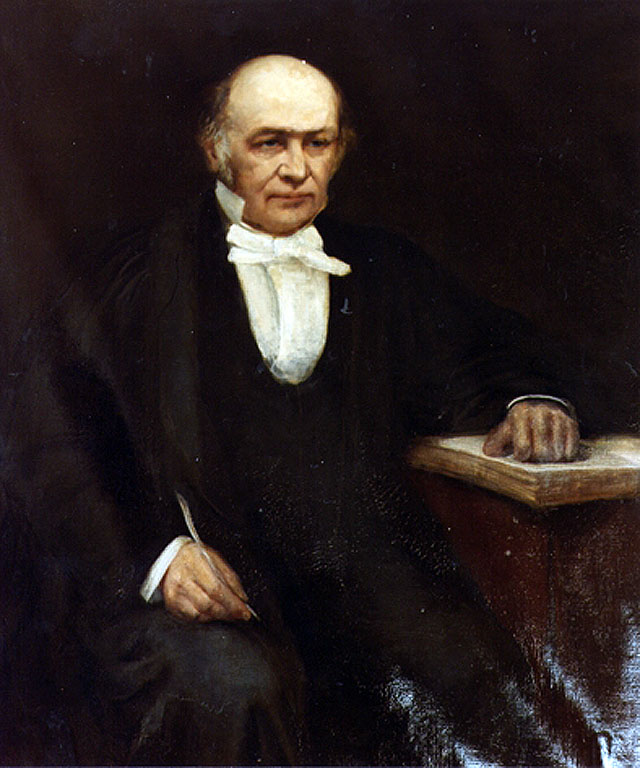
\includegraphics[width=0.8\textwidth]{hamilton_portrait.jpg}
                \caption{Sir William Rowan \textsc{Hamilton} \cite{hamilton_portrait}}
            \end{figure}
        \end{column}
        \end{columns}
    \end{frame}

    \begin{frame}
        \begin{columns}
        \begin{column}{0.5\textwidth}
            \begin{itemize}
                \item
                    Hamilton beschäftigt sich 1835 mit der geometrischen Bedeutung der \emph{komplexen Zahlen} im \(\R^2\)

                \item
                    Er fragt sich:
                    \enquote{Gibt es eine ähnliche Interpretation im \(\R^3\)?}
            \end{itemize}
        \end{column}
        \begin{column}{0.5\textwidth}
            \begin{figure}
                \includesvg[width=\textwidth]{komplexe_multiplikation}
                \caption{Geometrische Interpretation der komplexen Multiplikation \cite{komplexe_multiplikation}}
            \end{figure}
        \end{column}
        \end{columns}
    \end{frame}

    \begin{frame}
    \begin{columns}
    \begin{column}{0.5\textwidth}
        \begin{itemize}
            \item<1->
                Hamilton sucht eine Multiplikation, die die bisherigen Regeln und Beziehungen weiterhin erfüllt.

            \item<2->
                Erster Ansatz: \(x = \alpha + \beta i + \gamma j\) mit \(i^2 = j^2 = -1\).

            \item<3->
                Er stellt fest, dass für die Gültigkeit der Produktregel \(ij + ji = 0\) gelten muss.
                Unter Erhaltung der Kommutativität hieße dies: \(2ij = 0 \implies ij = 0\), was ihm aber nicht gefällt.
        \end{itemize}
    \end{column}
    \begin{column}{0.5\textwidth}
        \begin{beamercolorbox}[wd=\textwidth, rounded=true, shadow=true]{quote}
            \enquote{Well, Papa, can you multiply triplets?}

            \enquote{No, I can only add and subtract them.}

            \vspace{2mm}
            \hfill {\scriptsize--- Gespräch zwischen Hamilton und seinem Sohn}
        \end{beamercolorbox}

        \begin{itemize}
            \item<4->
                Stattdessen gibt Hamilton lieber die Kommutativität auf, was \(ji = -ij\) erlaubt.

            \item<5->
                Die entscheidende Idee kommt ihm 1843:\\
                Er setzt \(ij := k, ji = -k\) und nimmt  \(k\) als linear unabhängig von \(i\) und \(j\) an.
        \end{itemize}
        \vfill
    \end{column}
    \end{columns}
    \end{frame}

    \begin{frame}
        \begin{figure}
            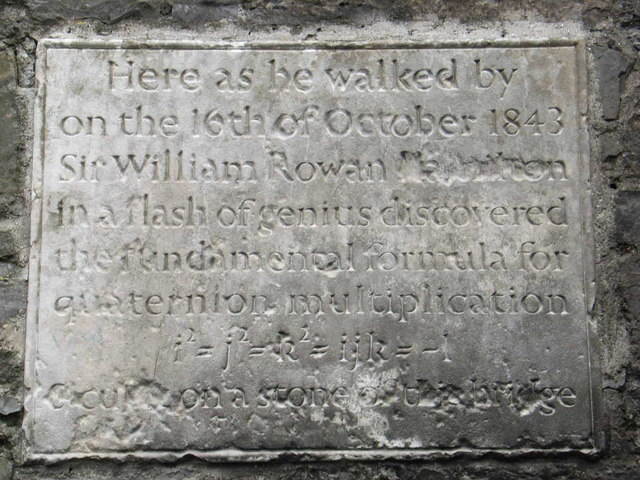
\includegraphics[width=0.7\textwidth]{broome_bridge.jpg}
            \caption{Gedenktafel an der \textit{Broome Bridge} in Dublin \cite{broome_bridge}}
        \end{figure}
    \end{frame}

    \section{Die Quaternionenalgebra \(\mathbb{H}\)}

    \begin{frame}
        Hamilton definiert die \emph{Quaternionen-Algebra} \(\Ham\) durch die Festlegung der Produkte der Basiselemente
        \[
            e_1 := (1,0,0,0), \, e_2 := (0,1,0,0), \, e_3 := (0,0,1,0), \, e_4 := (0,0,0,1):
        \] 
        \centering
        \begin{tabular}{crrr}
                    & \(e_2\) & \(e_3\) & \(e_4\) \\ \midrule
            \(e_2\) & \(- e_1\) & \(e_4\) & \(- e_3\) \\
            \(e_3\) & \(- e_4\) & \(- e_1\) & \(e_2\) \\
            \(e_4\) & \(e_3\) & \(- e_2\) & \(-e _1\)
        \end{tabular}

        \small (Es sei \(e_1\) das Einselement.)

        \raggedright
        \normalsize
        Man sieht direkt, dass \(\Ham\) nicht kommutativ ist.
        Die Assoziativität lässt sich wie im Einführungsabschnitt besprochen überprüfen.
    \end{frame}

    \begin{frame}
        Neben dieser klassischen Konstruktion von \(\Ham\) gibt es noch einen eleganteren Weg, der uns viele Eigenschaften der Quaternionen-Algebra direkter liefert:

        \begin{theorem}
            Die Menge 
            \[
                \mathcal{H} := \left\{ \begin{pmatrix} w & -z \\ \bar{z} & \bar{w} \end{pmatrix} 
                                        \colon w, z \in \mathbb{C} \right\}
            \] ist eine \(\mathbb{R}\)-Unteralgebra von \(\Mat(2, \mathbb{C})\) mit Einselement \(E_2\).

            Jede Matrix \(A \in \mathcal{H}\) genügt der Gleichung
            \[
                A^2 - (\spur A) A + (\det A) E = 0
            .\] 

            \(\mathcal{H}\) ist eine vierdimensionale, assoziative Divisionsalgebra.
        \end{theorem}
    \end{frame}

    \begin{frame}
        \begin{proof}
            \only<1>{
            Man verifiziert durch Nachrechnen, dass \(\mathcal{H}\) ein vierdimensionaler \(\mathbb{R}\)-UVR von \(\Mat(2, \mathbb{C})\) ist.
            Auch die Abgeschlossenheit bezüglich der Matrizenmultiplikation überprüft man auf diese Weise.

            Die angegebene Gleichung ist ein Spezialfall des Satzes von Cayley-Hamilton.

            Die Assoziativität ist klar, da \(\Mat(2, \mathbb{C})\) assoziativ ist.
            }
            \only<2>{
            Um einzusehen, dass \(\mathcal{H}\) auch eine Divisionsalgebra ist, benutzen wir das eingangs bewiesene Nullteilerkriterium:\\
            Seien also \(A, B \in \mathcal{H}\) mit \(AB = 0\).
            Wegen des Determinantenmultiplikationsatzes gilt \(\det(A) \cdot \det(B) = 0\), also \(\det(A) = 0\) oder \(\det(B) = 0\).
            Aus
            \[
                \det \begin{pmatrix} w & -z \\ \bar{z} & \bar{w} \end{pmatrix} = \abs{w}^2 + \abs{z}^2 = 0 \iff w = z = 0
            \]
            folgt
            \[
                AB = 0 \iff A = \begin{pmatrix} 0 & 0 \\ 0 & 0 \end{pmatrix} \text{ oder } B = \begin{pmatrix} 0 & 0 \\ 0 & 0 \end{pmatrix}
            .\] 
            Das bedeutet, dass \(\mathcal{H}\) keine Nullteiler \(\neq 0\) besitzt.
            Damit ist \(\mathcal{H}\) eine Divisionsalgebra.
            }
            \alt<2>{\qedhere}{\phantom\qedhere}
        \end{proof}
    \end{frame}

    \begin{frame}
        \begin{lemma}
            Die Abbildung
            \[
                F \colon \Ham \to \mathcal{H}, \quad (\alpha, \beta, \gamma, \delta) \mapsto
                    \begin{pmatrix}
                        \alpha + \beta i  & - \gamma - \delta i \\
                        \gamma - \delta i & \alpha - \beta i
                    \end{pmatrix}
            ,\]
            ist ein \(\mathbb{R}\)-Algebra-Isomorphismus und es gilt:
            \begin{align*}
                F(e_1) = E_2 =: E,& \quad
                F(e_2) = \begin{pmatrix} i & 0 \\ 0 & -i \end{pmatrix} =: I, \\
                F(e_3) = \begin{pmatrix} 0 & -1 \\ 1 & 0 \end{pmatrix} =: J,& \quad
                F(e_4) = \begin{pmatrix} 0 & -i \\ -i & 0 \end{pmatrix} =: K.
            \end{align*}
        \end{lemma}
    \end{frame}

    \begin{frame}
        \begin{cor}
            Die Hamiltonsche Algebra \Ham ist eine assoziative Divisionsalgebra.
        \end{cor}

        \uncover<2>{
        \begin{proof}
            Wir haben gezeigt, dass \(\mathcal{H}\) eine assoziative Divisionsalgebra ist.

            Durch den oben beschriebenen Isomorphismus \(F\) ist also auch \Ham eine assoziative Divisionsalgebra.
        \end{proof}

        \vfill
        Man muss also \enquote{nur} mit komplexen Matrizen rechnen können, um den Umgang mit der Quaternionen-Algebra zu beherrschen.
        }
    \end{frame}

    \section{Der Imaginärraum von \(\mathbb{H}\)}
    \begin{frame}
        \begin{definition}
            Der Untervektorraum
            \[
                \Im(\Ham) := \R i + \R j + \R k
            \]
            heißt \emph{Imaginärraum}.
            Seine Elemente werden auch als vektorielle Quaternionen bezeichnet.

            Äquivalent zu dieser (basisabhängigen) Darstellung ist die Form
            \[
                \Im(\Ham) = \left\{ x \in \Ham \colon x^2 \in \R e \text{ und } x \notin \R e \setminus \left\{ 0 \right\} \right\}
            .\] 
        \end{definition}

        Aus dieser Darstellung folgert man, dass es zu jedem \(u \in \Im(\Ham), \, u \neq 0,\) einen Skalar \(\varrho\) mit \((\varrho u)^2 = - e\) gibt.
        (Man kann also normieren.)

        Wegen \(x^2 \in \R e \nsubseteq \Im(\Ham)\) ist \(\Im(\Ham)\) keine \(\R\)-Unteralgebra von \(\Ham\).
    \end{frame}

    \begin{frame}
        Wir wollen zeigen, dass die beiden Darstellungen tatsächlich übereinstimmen.

        Sei \(x \in \Ham\).
        Wir setzen \(F(x) =: X \in \mathcal{H}\).
        Wie oben besprochen erfüllt jede solche Matrix den Satz von Cayley-Hamilton:
        \begin{alignat*}{3}
                 &&X^2 - 2 \alpha X + \left( \alpha^2 + \beta^2 + \gamma^2 + \delta^2 \right) E &= 0 \\
            \iff &&X^2 &= 2 \alpha X - \left( \alpha^2 + \beta^2 + \gamma^2 + \delta^2 \right) E \\
            \iff &&x^2 &= 2 \alpha x - \left( \alpha^2 + \beta^2 + \gamma^2 + \delta^2 \right) e
        \end{alignat*}
        Sei jetzt \(\Im(\Ham)\), also \(\alpha = 0\).
        Daher
        \[
            x^2 = \underbrace{- \left( \beta^2 + \gamma^2 + \delta^2 \right)}_{\in \, \R} e \iff x^2 \in \R e
        ,\] 
        und das zeigt die Behauptung.
    \end{frame}

    \begin{frame}
        Jedes Quaternion \(x \in \Ham\) besitzt also eine eindeutige Darstellung
        \[
            x = \alpha e + u \quad \text { mit } \quad \alpha \in \R \text{ und } u \in \Im(\Ham)
        .\]
        Man nennt
        \begin{itemize}
            \item 
                \(\alpha e\) \emph{skalaren Anteil} oder \emph{Realteil}, und 

            \item
                \(u\) \emph{vektoriellen Anteil} oder \emph{Imaginärteil}
        \end{itemize}
        von \(x\).

    \end{frame}

    \subsection{Quaternionenmultiplikation}

    \begin{frame}
        Seien
        \[
            u = \beta i + \gamma j + \delta k,
            \quad v = \varrho i + \sigma j + \tau k
            \quad \in \Im(\Ham) \cong \R^3
        .\]
        Durch Ausmultiplizieren ergibt sich
        \[
            uv = - (\beta \varrho + \gamma \sigma + \delta \tau) e + (\gamma \tau - \delta \sigma) i + (\delta \varrho - \beta \tau) j + (\beta \sigma - \gamma \varrho) k
        .\]
        Dies kann man auch schreiben als
        \[
            uv = - \langle u, v \rangle e + u \times v
        ,\] 
        und gewinnt so auf natürliche Weise Skalar- und Kreuzprodukt aus der Quaternionenmultiplikation.
    \end{frame}

    \begin{frame}
        Für \(u, v, w \in \Im(\Ham)\) bestätigt man durch einfaches Nachrechnen:
        \begin{itemize}
            \item
                \(u \times v = \frac{1}{2} (uv - vu)\)

            \item
                \(\langle v, u \rangle e = - \frac{1}{2} (uv + vu)\)

            \item
                \(u \times (v \times w) = \frac{1}{2} (uvw - vwu)\)

            \item
                \(\langle u, v \rangle^2 + \abs{u \times v}^2 = \abs{u}^2 \abs{v}^2\)

            \item
                \(\langle u \times v, w \rangle = \langle u, v \times w \rangle\) \hfill (Vertauschungsregel)

            \item
                \(u \times (v \times w) = \langle u, w \rangle v - \langle u, v \rangle w\) \hfill (\textsc{Grassmann}-Identität)

            \item
                \(u \times (v \times w) + v \times (w \times u) + w \times (u \times v) = 0\) \hfill (\textsc{Jacobi}-Identität)
        \end{itemize}
    \end{frame}

    \section{Zentrum von \(\mathbb{H}\)}
    \begin{frame}
        \begin{definition}
            Für eine Algebra \(\mathcal{A}\) heißt
            \[
                Z \left( \mathcal{A} \right) := \left\{ z \in \mathcal{A} \colon zx = xz \text{ für alle } x \in \mathcal{A} \right\}
            \] 
            \emph{Zentrum} von \(\mathcal{A}\).
            Es handelt sich also um diejenigen Elemente in \(\mathcal{A}\), die mit allen Elementen kommutieren.

            Ist \(\mathcal{A}\) assoziativ, so ist \(Z(\mathcal{A})\) eine Unteralgebra von \(\mathcal{A}\).
            Falls \(\mathcal{A}\) kommutativ ist, so ist \(Z(\mathcal{A}) = \mathcal{A}\).
            Ist \(\mathcal{A}\) eine Algebra mit Einselement, so ist trivialerweise \(\R e \subseteq Z(\mathcal{A})\).
        \end{definition}
    \end{frame}

    \begin{frame}
        \begin{theorem}
            Für die Algebra \Ham gilt \(Z \left( \Ham \right) = \R e\).
        \end{theorem}
    \end{frame}

    \begin{frame}
        \begin{proof}
            \only<1>{
            Es ist klar, dass \(\R e \subseteq Z \left( \Ham \right) \); denn  \(e\) ist neutrales Element, also per Definition mit allen Elementen aus \(\Ham\) kommutativ.
            Die Skalare sind natürlich ebenfalls kommutativ zueinander.
            }
            \only<2>{
            Zur Umkehrung.\\
            Sei \(x = \alpha e + \beta i + \gamma j + \delta k \in Z \left( \Ham \right)\), das heißt, \(x\) kommutiert mit allen Elementen aus \(\Ham\).
            Insbesondere kommutiert \(x\) mit den Basiselementen \(i, \, j \in \Ham\), es muss also \(ix = xi\) und \(jx = xj\) gelten.

            Wir wollen zeigen, dass dann bereits \(x \in \R e\) ist.
            }
            \only<3>{
            Ausmultiplizieren der ersten Gleichung ergibt
            \begin{alignat*}{3}
                     &&xi &= ix \\
                \iff &&\alpha i - \beta + \gamma k - \delta j &= \alpha i - \beta - \gamma k + \delta j \\
                \iff &&\gamma k - \delta j &= - \gamma k + \delta j \\
                \iff &&\gamma k - \delta j &= - (\gamma k - \delta j) \\
                \iff &&2 \gamma k - 2 \delta j &= 0 \\
                \iff &&\gamma = \delta &= 0.
            \end{alignat*}
            }
            \only<4>{
            Analog ergibt sich aus der zweiten Gleichung \(\beta = \delta = 0\).
            Damit ist \(\beta = \gamma = \delta = 0\).
            \(x\)~ist demnach von der Form \(x = \alpha e\), also \(x \in \R e\).
            Das bedeutet \(Z \left( \Ham \right) \subseteq \R e\), und damit folgt zusammen mit dem ersten Teil wie gewünscht
            \[
                Z \left( \Ham \right) = \R e
            .\]
            }
            \alt<4>{\qedhere}{\phantom\qedhere}
        \end{proof}
    \end{frame}

    % Diese Sektion auslassen?
    \section{Endomorphismen von \(\mathbb{H}\)}
    \begin{frame}
        Es sei \(\End(\Ham)\) der \(\R\)-Vektorraum aller Endomorphismen von \(\Ham\).

        \begin{theorem}
            Ist \(a_1, \dots, a_4\) eine Basis von \(\Ham\), so ist die Abbildung
            \[
                F \colon \Ham^4 \to \End(\Ham), \quad \left( b_1, b_2, b_3, b_4 \right) \mapsto f \in \End(\Ham) \text{ mit } f(x) := \sum_{i=1}^4 a_i x b_i
            \] 
            \(\R\)-linear und bijektiv.

            Es lässt sich (bei fixierter Basis) also jeder Endomorphismus von \Ham eindeutig durch ein Tupel \(\left(b_1, \dots, b_4\right)\) identifizieren.
        \end{theorem}
    \end{frame}

    \begin{frame}
        \begin{proof}
            \only<1>{
            Die \(\R\)-Linearität sieht man schnell ein.

            Da \(\dim\left(\Ham^4\right) = \dim\left(\End\left(\Ham\right)\right) = 16 < \infty\), braucht man nur die Injektivität zeigen.
            Dann folgt aus der Dimensionsformel die Surjektivität und damit auch die Bijektivität.
            Für den Beweis der Injektivität benutzen wir das Kernkriterium.

            Dazu zeigen wir die Hilfsaussage:
            \begin{center}
                Sei \(n = 1, 2, 3, 4\), sei \(f_n(x) = \sum_{i=1}^n a_ixb_i = 0\) für alle \(x \in \Ham\).\\
                Dann gilt \(b_1 = \dots = b_n = 0\).
            \end{center}
            }
            \only<2>{
                Wir gehen induktiv vor, der Fall \(n = 1\) ist klar.
                Sei also \(n > 1\).
                In der Absicht, einen Widerspruch zu erhalten, nehmen wir \(b_1 \neq 0\) an:
                \[
                    a_1 x + \sum_{i=2}^n a_i x q_i = 0 \quad \text{ mit } q_i := b_i b_1^{-1}
                .\] 
                Da \(f_n(x) = 0\) für alle \(x \in \Ham\), gilt:
                \begin{alignat*}{3}
                    &&f_n(x) y = 0 &= f_n(xy) \\
                    \iff &&a_1 x y + \sum_{i=2}^n a_i x q_i y &= a_1 x y + \sum_{i=2}^n a_i x y q_i \\
                    \iff &&\sum_{i=2}^n a_i x (q_i y) - \sum_{i=2}^n a_i x (y q_i) &= 0 \\
                    \iff &&\sum_{i=2}^n a_i x (q_i y - y q_i) &= 0
                \end{alignat*}
            }
            \only<3>{
                Da die \(a_i\) Basiselemente sind, ist \(a_i \neq 0\) für alle \(i = 1, \dots, 4\).
                Deswegen muss
                \[
                q_i y - y q_i = 0 \iff q_i y = y q_i
                \] 
                für alle \(y \in \Ham\) gelten.

                Damit ist \(q_i \in Z(\Ham) = \R e\) nach dem vorherigen Abschnitt, also
                \[
                    q_i = \alpha_i e \quad \text{ mit } \quad \alpha_i \in \R
                .\] 
            }
            \only<4>{
                Einsetzen in die Ausgangsgleichung ergibt
                \begin{alignat*}{3}
                    &&a_1 x + \sum_{i=2}^n a_i x q_i &= 0 \\
                    \iff &&a_1 x + \sum_{i=2}^n \alpha_i a_i x &= 0 \\
                    \iff &&\left( a_1 + \sum_{i=2}^n \alpha_i a_i \right) x &= 0 \\
                    \iff &&a_1 + \sum_{i=2}^n \alpha_i a_i &= 0.
                \end{alignat*}
            }
            \only<5>{
                Dann wären die \(a_1, \dots, a_4\) linear abhängig, was aber aufgrund der Basiseigenschaft ein Widerspruch ist.

                Also muss doch \(b_1 = 0\).
                Analog erhält man \(b_2 = b_3 = b_4 = 0\).

                Damit ist der Kern von \(F\) trivial; also ist \(F\) injektiv und nach der Dimensionsformel auch bijektiv.
            }
            \alt<5>{\qedhere}{\phantom\qedhere}
        \end{proof}
    \end{frame}

    \begin{frame}
        Wir geben ein Beispiel für einen Endomorphismus.
        Die \emph{Konjugierung}
        \[
            \Ham \to \Ham, \quad
            x = \alpha e + \beta i + \gamma j + \delta k \mapsto \bar{x} = \alpha e - \beta i - \gamma j - \delta k
        \]
        wird bezüglich der Standardbasis \(e, i, j, k\) beschrieben durch
        \begin{align*}
            \bar{x} &= - \half \left( x + ixi + jxj + kxk \right) \\
                    &= - \half exe - \half ixi - \half jxj - \half kxk \\
                    &= F \left( - \half e, \, - \half i, \, - \half j, \, - \half k \right),
        \end{align*}
        und dies ist offensichtlich von der Form des vorherigen Satzes.
    \end{frame}

    \section{Bezug zur Vektoranalysis}

    \begin{frame}
        Mithilfe der Quaternionenmultiplikation lassen sich einige bekannte Operatoren der Vektoranalysis elegant herleiten.

        \begin{definition}
            Der \textit{Nabla-Operator} wird definiert durch
            \[
                \nabla := \diff{}{x} i + \diff{}{y} j + \diff{}{z} k
            .\]
        \end{definition}
    \end{frame}

    \begin{frame}
        Sei \(f \colon \R^3 \to \R\) eine differenzierbare Funktion.
        Die Anwendung des Nabla-Operators liefert
        \[
            \nabla f = \diff{f}{x} i + \diff{f}{y} j + \diff{f}{z} k = \grad \left( f \right)
        .\]

        Zweimalige Anwendung von \(\nabla\) liefert den Laplace-Operator \(\Delta\):
        \[
            \nabla^2 f = - \left( \lap{f}{x} + \lap{f}{y} + \lap{f}{z} \right) = - \Delta f 
        .\]
    \end{frame}

    \begin{frame}
        Sei
        \[
            F \colon \R^3 \to \Im \left( \Ham \right),
            (x,y,z) \mapsto u(x,y,z) i + v(x,y,z) j + w(x,y,z) k
        .\]
        Anwendung von \(\nabla\) liefert
        \[
            \nabla F = - \left( \diff{u}{x} + \diff{v}{y} + \diff{w}{z} \right) e
            + \left( \diff{w}{y} - \diff{v}{z} \right) i
            + \left( \diff{u}{z} - \diff{w}{x} \right) j
            + \left( \diff{v}{x} - \diff{u}{y} \right) k
        ,\]
        das heißt
        \[
            \nabla F = - \left( \newdiv F \right) e + \rot F
        .\]
    \end{frame}

    \section{Fundamentalsatz der Algebra für Quaternionen}

    \begin{frame}
        \begin{theorem}[\textsc{Eilenberg} und \textsc{Niven}, 1944]
            Sei \(p\) ein Polynom über \Ham vom Grad \(n > 0\) mit der Form \(p = m + q\), wobei \(m\) ein Monom vom Grad \(n\), und \(q\) ein Polynom vom Grad \(< n\) ist.
            Dann ist die Abbildung \(p \colon \Ham \to \Ham\) surjektiv; besitzt also insbesondere Nullstellen in \(\Ham\).
        \end{theorem}

        \uncover<2>{
        Der Satz verliert seine Gültigkeit, sobald es mehrere Polynome höchsten Grades in \(p\) gibt.
        So besitzt zum Beispiel \(iX - Xi + 1\) keine Nullstellen in \(\Ham\).
        }
    \end{frame}

    \begin{frame}
        \begin{proof}
            Leider nicht mit ähnlichen Methoden wie für \(\mathbb{C}\) beweisbar.  
            Mit topologischen Hilfsmitteln:

            Da in \(p\) das Monom \(n\)-ten Grades für große \(x \in \Ham\) dominiert, gilt
            \[
                \lim_{x \to \infty} \abs{p(x)} = \infty
            .\]
            Daher ist \(p\) zu einer stetigen Abbildung \(\hat{p} \colon S^4 \to S^4\) der vierdimensionalen Sphäre in sich mit \(\hat{p} := \infty\) fortsetzbar (man fasse \(S^4\) als die Kompaktifizierung von \(\Ham \cong \R^4\) durch einen Punkt \(\infty\) auf).
            Nun lässt sich zeigen, dass \(\hat{p}\) den topologischen Abbildungsgrad \(n\) hat.
            Da \(n \neq 0\) nach Voraussetzung, so ist \(\hat{p}\) nach einem Satz der Topologie surjektiv.
        \end{proof}
    \end{frame}

    \begin{frame}[allowframebreaks]
        \printbibliography[title={Quellen \& Verweise}]
    \end{frame}
\end{document}
